\begin{figure}[h!]
\centering
% Thesis-wide categorical color palette
% Usage: % Thesis-wide categorical color palette
% Usage: % Thesis-wide categorical color palette
% Usage: \input{figures/palette} in any figure file
%
% Muted primary colors -- print-friendly, visually distinct.
% Inspired by Cooper Union's red/blue primaries, softened for
% academic figures. Use palA-palC for data series in scatter
% plots, line charts, bar charts, etc.

\definecolor{palA}{HTML}{1F77B4}   % Tableau blue
\definecolor{palB}{HTML}{D62728}   % Tableau red
\definecolor{palC}{HTML}{2CA02C}   % Tableau green
 in any figure file
%
% Muted primary colors -- print-friendly, visually distinct.
% Inspired by Cooper Union's red/blue primaries, softened for
% academic figures. Use palA-palC for data series in scatter
% plots, line charts, bar charts, etc.

\definecolor{palA}{HTML}{1F77B4}   % Tableau blue
\definecolor{palB}{HTML}{D62728}   % Tableau red
\definecolor{palC}{HTML}{2CA02C}   % Tableau green
 in any figure file
%
% Muted primary colors -- print-friendly, visually distinct.
% Inspired by Cooper Union's red/blue primaries, softened for
% academic figures. Use palA-palC for data series in scatter
% plots, line charts, bar charts, etc.

\definecolor{palA}{HTML}{1F77B4}   % Tableau blue
\definecolor{palB}{HTML}{D62728}   % Tableau red
\definecolor{palC}{HTML}{2CA02C}   % Tableau green

\definecolor{agentblue}{HTML}{4C72B0}
\definecolor{rewardgreen}{HTML}{55A868}
\definecolor{penaltyred}{HTML}{C44E52}

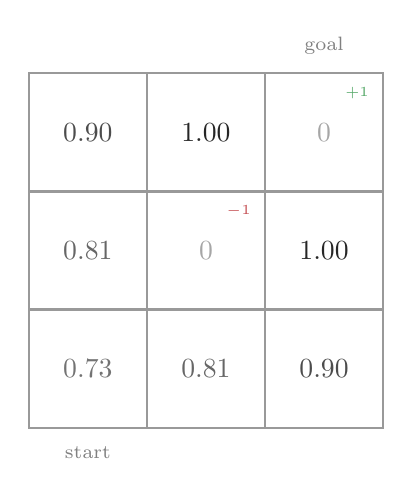
\begin{tikzpicture}[
    cell/.style={minimum size=1.5cm, draw=black!40, thick},
    val/.style={font=\normalsize},
    reward/.style={font=\normalsize\bfseries},
    agent/.style={circle, draw=agentblue, thick,
                  fill=agentblue!20, inner sep=3.5pt},
]
\def\s{1.5}

% Grid
\foreach \x in {0,1,2} {
    \foreach \y in {0,1,2} {
        \node[cell] (c\x\y) at (\x*\s, \y*\s) {};
    }
}

% Values
\node[val, text=black!55] at (c00) {0.73};
\node[val, text=black!60] at (c10) {0.81};
\node[val, text=black!70] at (c20) {0.90};
\node[val, text=black!60] at (c01) {0.81};
% s_11: penalty (terminal, v=0, reward shown in corner)
\node[val, text=black!35] at (c11) {0};
\node[font=\tiny\bfseries, text=penaltyred, anchor=north east]
    at ([xshift=-2pt, yshift=-2pt]c11.north east) {$-1$};

\node[val, text=black!85] at (c21) {1.00};
\node[val, text=black!70] at (c02) {0.90};
\node[val, text=black!85] at (c12) {1.00};

% s_22: goal (terminal, v=0, reward shown in corner)
\node[val, text=black!35] at (c22) {0};
\node[font=\tiny\bfseries, text=rewardgreen, anchor=north east]
    at ([xshift=-2pt, yshift=-2pt]c22.north east) {$+1$};


% Labels
\node[font=\scriptsize, text=black!50, below=3pt]
    at (c00.south) {start};
\node[font=\scriptsize, text=black!50, above=3pt]
    at (c22.north) {goal};

\end{tikzpicture}

\vspace{0.5em}
\caption{State values $v_\pi(s)$ in the grid-world ($\gamma = 0.9$).
  Values increase with proximity to the goal; terminal cells have
  $v = 0$ (corner labels show the entry reward).}
\label{fig:value-grid}
\end{figure}
